%++++++++++++++++++++++++++++++++++++++++
% Don't modify this section unless you know what you're doing!
\documentclass[letterpaper,12pt]{article}
\usepackage{tabularx} % extra features for tabular environment
\usepackage{amsmath}  % improve math presentation
\usepackage{graphicx} % takes care of graphic including machinery
\usepackage[margin=1in,letterpaper]{geometry} % decreases margins
\usepackage{cite} % takes care of citations
\usepackage[final]{hyperref} % adds hyper links inside the generated pdf file
\hypersetup{
	colorlinks=true,       % false: boxed links; true: colored links
	linkcolor=blue,        % color of internal links
	citecolor=blue,        % color of links to bibliography
	filecolor=magenta,     % color of file links
	urlcolor=blue         
}
%++++++++++++++++++++++++++++++++++++++++


\begin{document}
	
	\title{COMP 512 Final Project Report}
	\author{Yiwei Xia and Marie Payne}
	\date{\today}
	\maketitle
	
	\pagebreak
	
	\section{Introduction}
	
	The goal of our project is to design and develop a distributed system where clients can make requests and servers deliver responses based upon them, with the use of a middleware server, as well as servers to manage the locking mechanisms and transaction implementation. The aim is to develop this system using the Transmission Control Protocol (TCP), and to make it robust to system failures, and to uphold data integrity through data persistance.
	
	
	\section{Design}

	\subsection*{RMI and TCP}  

	Initially, for both TCP and RMI implementations, the middleware server implemented the resource manager interface, but also acted as a client. This was done so that from the point of view of the client, the middleware is a just another resource manager, and from the point of view of the resource manager, the middleware is another client. This allowed for maximum code reuse, as the middleware became a sort of amalgamation of the original client and resource managers.\\

	For TCP, the ports for the RM servers for each resource (car, flight, hotel rooms, customers) are hard-coded. Calling a remote method was done by wrapping the functions into request objects using the command pattern, and passing these request objects to the remote server, and waiting for a reply object. The objects were sent from machine to machine via TCP by first serializing them into a JSON string using the Jackson object mapper library. \\

	Since each of the requests on the middleware was blocking, each request was run on a new thread so as to allow other clients to make requests to the middleware in the meantime.\\

	Our original system consisted of 1 client, 1 middleware, and 4 RMs, one each for flights, cars, hotels, and customers.\\

	\subsection*{Transactions}

	For Transactions and Replication, TCP was used instead of RMI.\\
	
	Implementing locks and transactions required a change to the ResourceManager interface. However, no new functionality was needed to communicate between the middleware and the RMs. Instead of modifying middleware-RM communications to accomodate functionality it didn't need, a new interface was created called TransactionalResourceManager, which implemented the start, commit, abort functions. Naturally, there is also a new TransactionalMiddleware, which accepts the new start, commit, abort functions.\\
	
	Locking is managed by a LockManager. This manager is different from the provided one in that it doesn't differentiate between timeouts/deadlocks and acquired/redundant locks. When the middleware requests a lock on an object, it simply returns true within the timeout (10 seconds) if the lock has been acquired, or false once that time limit has been reached. This puts the responsibility of deciding whether or not a deadlock has happened on the middleware. The client is not aware of locks. Locks are acquired by the middleware automatically as needed for each function call, and released after commit/abort, as per 2PL.\\
	
	Transactions are managed by a TransactionManager. The TransactionManager has a stack of ``requests'' for each transaction, and supports 4 functions: start, commit, abort, and addRequest. The stack of requests keep track of the changes needed to revert the RMs back to their original states in case of an abort. Everytime the middleware performs a modification, i.e. a write, it calls addRequest to and pushes opposite request to the stack for that transaction in the transaction manager. \\
	
	For example, if the client requests createResource(), the transactionalMiddleware will first lock the necessary resource. Then, it will create the resource on the appropriate RM, and then will push a deleteResource() request to the transaction stack in the transaction manager. If the transactionalMiddleware were to fail at this point, and was irrecoverable, the change would have effectively been committed. However, since we're assuming no failures, this is not a problem. Now, if a commit message is sent, the changes are already in the RMs, the transacation manager clears the stack for that transaction, and no more work is needed. However, in the case of a deadlock/abort situation, the transaction will pop every request in the stack, restoring the RMs into their original condition. Because 2 phase locking is used, popping the entire stack is guaranteed to return the RMs to their original conditions.\\
	
	In order to push functions onto stacks, the command pattern was used to create two sets of classes in accordance to the the ResourceManager and TransactionalResourceManager interfaces.\\
	
	With the way aborts work, it was necessary to create ''doubles'' of each function. If the TransactionalMiddleware create() function were to push the TransactionalMiddleware delete() function onto the stack, popping that delete function would push a create() function onto the stack, making an endless loop. Instead, the TransactionalMiddleware create() function pushes the Middleware delete() function onto the stack, whose operations are final (the same way they were implemented in project one).\\

    \subsection*{Replication}

    For replication, the implementation used 2 instances of each ``class'', which is a piece of the distributed system. The middleware, customer RM, car RM, flight RM, and hotel RM are each an individual class.\\

    In order to be fault tolerant, the state of all instances in a class should be consistent with eachother at all times. This way, when one instance crashes, the remaining instances are all complete and correct, and would be able to continue on without the failed one. For this purpose, JGroups were used instead of using sockets with TCP. Jgroups has multiple protocols for communication, and can not only guarantee delivery, but have total ordering for delivery for all messages in that channel. Because of this, it is ensured that every receiver receives messages in the same order. The receivers were implemented so that they would all execute the requests sequentially in the order they were received. This way, since all the machines start in the same state, all the same requests are applied to all machines in the exact same order, and all requests are deterministic, the state of all the machines must be the same.\\

    Communication was implemented by having two channels between any two communicating classes, the request channel and the reply channel. There would be a request channel, and a reply channel. Each request that is sent from client to middleware, or middleware to RM, has an associated requestId, determined by an incrementing count on the sending machine. This requestId is used to distinguish duplicate messages, and ensure that no action is performed twice. There is no need to sync the requestId between middlewares, as the counters both start at the same number, and increment the exact same with each request that passes through it. After the message is sent on the request channel, the sender checks a reply queue for the reply with the same requestId.\\

    JGroups have a ``receiver adapter'' class, which has a function to be overridden called ``receive''. When any instance receives a message from a channel it is receiving in, it first checks to see if this requestId has already been received. If it has, it discards the message. It it hasn't it adds it to the queue. In this way, it doesn't matter if there is 1 instance of each class or 1000, as for each requestId, only the first request/reply for that requestId is processed. This works because the system makes no distinction between requests/replies sent by instances of the same class.\\

    For example, the client can request to update a car resource. It will send a this request to the client-middleware channnel. Both middleware 1 and middleware 2 will receive this request, and will both send an updateResource request in the middleware-carRm-request channel. Both of the car Rms will receive both of these messages. However, say middleware 2 managed to send its message to the channel first. Because of the total ordering property of the JGroup channel, both rms will receive the request from middleware 2, and will perform the action. Later on, they will receive an identical requset from middleware 1, which they will then discard. They will then both proceed to send a reply to the middleware-carRm-reply channel. Whichever RM manages to send first will have their message picked up by both middlewares first. They will then return that same reply along to the client in the client-middleware channel. Once again, both will send it, but only the first message will get picked up by the Client.\\ 

	\begin{center} 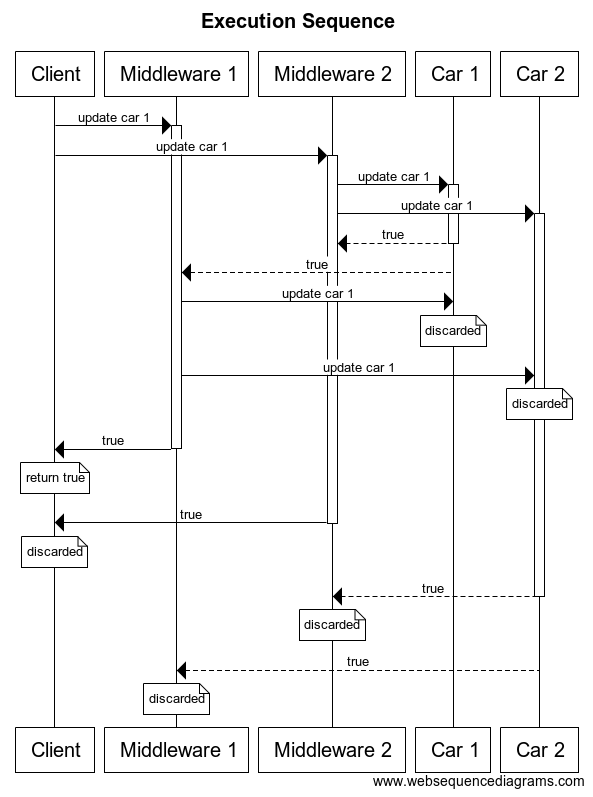
\includegraphics[width=0.8\columnwidth]{Execution_Sequence.png}
	\end{center}

	\pagebreak

	\section{Special Features}

	The provided code was refactored into kotlin in order to speed up development. The lockmanager class was recoded from scratch to not have two waiting queues, and is much more readable and easy to understand.

	\section{Optimistic Concurrency Control}

	In the case of optimistic concurrency control, the entire system would need to be refactored to return copies of resources and customers. No locks would be used, and instead, copies of objects would be returned with version numbers, and before committing, these version numbers would have to be atomically checked with resource managers to ensure that they were still consistent. If not, the transaction would be forced to abort, discarding its changes. 

	\section{Problems}

	Initially there was some difficulty with how to perform the TransactionManager's undo stack, as originally it would call the opposite method in the TransactionalMiddleware. That method would push its own undo function onto the stack as well, creating an infinite loop in case of an abort. It was solved by having two different middlewares, one whose functions had the undo, and one whose functions didn't. These became the TransactionalMiddleware and Middleware classes respectively. 

	\section{Testing}

	No testing framework was used, but there was a Tester class that used a client to programatically send a series of requests to the middlewares and checked the final state to ensure that things were working correctly. Furthermore, the extensive use of print statements was used, printing diagnostic messages and showing what json messages were passed between which instances. These were commented out for the demo, but still exist in the code. 
	
	\section{Performance Analysis Methods}
	
	The performance analysis we conducted on our system included two parts; the first part involving one client and the average response times of different API methods in the system, the second involving muliple clients and varying loads to analyze the response times. Since we're focusing on response times, we want to avoid deadlocking the system as much as possible, which can be done with multiple clients by only using one method, query, which has no possibility of deadlock even called in concurrence (multiple read locks can be acquired at once, in our implementation). \\
	
	The first part of the performance analysis simulated one customer on a loop. Every iteration of the program would choose a method and call it N times to produce an average, and print the response time on the customer side. Doing this narrows down the time spent at each stage in the method call on average, and can thus be used to figure out the bottleneck of the system and analyze where measures to increase efficiency can be implemented.\\
	
	The second part of the analysis simulates multiple customers in a number of threads, and calls methods selected so as to avoid creating a deadlock in a loop. The load is then varied from 1 to 10 (the threads sleep at a time interval adjusted to reflect this) and the average response time recorded. This is then plotted using matplotlib in Python to illustrate the results (each line is for the number of customers, best-fit). This part of the performance analysis is meant to determine the saturation point of the system, with some level of concurrency. However, this test uses an optimal system with no occurrence of deadlocks, when in reality this system will deadlock somewhat frequently when the number of client threads running increases. 
	
	\section{ Performance Analysis Results}
	The results for phase 1 of the performance analysis testing can be resolved in the following table:
	
	\begin{center}
		\begin{tabular}{ |c|c| } 
			\hline
			Method Call: & Client Side (ms) \\
			\hline
			start & 5.43  \\ 
			commit & 5.48  \\ 
			abort & 5.49  \\ 
			createResource & 10.64  \\ 
			updateResource & 10.22  \\ 
			reserveResource & 7.74  \\ 
			deleteResource & 8.85  \\ 
			queryResource & 5.52  \\ 
			uniqueCustomerId & 5.56  \\ 
			createCustomer & 10.78 \\
			queryCustomer & 11.75 \\ 
			deleteCustomer & 10.60 \\ 
			customerAddReservation & 10.94 \\ 
			customerRemoveReservation & 16.44 \\
			itinerary & 42.20\\
			\hline
		\end{tabular}\\
		Figure 1: Averages of method calls in the system in \\milliseconds, using one client and ideal conditions.
	\end{center}
	The method calls were performed in ideal contexts. The itinerary method was called using two resources chosen at random (this is sufficiently varied for our purposes, however it should be noted that using a larger itinerary will scale the average response time linearly with the resource managers used). Each average was taken by running the method call 100 times and averaging the total time, which ended up being overly cautious and unnecessary but smoothed out any minor discrepancies. Running the loops multiple times revealed a standard deviation of +- 0.30 ms, roughly (more testing could be done at this phase to determine the exact standard devation, though this precision is not necessary in the preliminary development phases of this system).\\
	
	The results for the second phase of the analysis are demonstrated in the figure shown:\\

	\begin{figure}[ht] 
		\centering 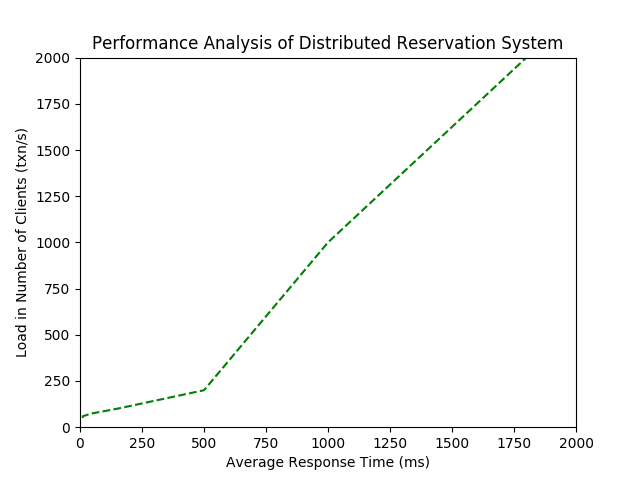
\includegraphics[width=0.8\columnwidth]{performanal.png}
	\end{figure}

	The only method used in the trials was queryResource, with a lot of instantiated resources that get queried randomly so to prevent the threads from simultaneously accessing the list data structures (this throws a data corruption error). Threads sleep before checking if responses are received, so <10 ms response times are not achievable.
	
	\section{Performance Analysis Discussion}
	For the first part of the performance testing, we used one client on a loop and took the average response time on the client side of each method available in the API. Several of the methods hovered around 10ms or below on average, with the exceptions of customerRemoveReservation and itinerary. These two methods used the most TCP calls compared to the other methods, which were more localized to one resource manager and performed checks against locally stored hashmaps and mutable lists. The performance of itinerary depends on a couple of variables, such as the number of resource managers involved, the number of resource IDs involved, and the size of the mutable map of resources being sent to the middleware server. The testing protocols used randomized two resources equally chosen from the three resource pools, so the reservable item mutable map being passed was a constant size, though the number of resource managers involved could vary. The standard deviation for this method was also larger, but if we accounted for the number of resource managers involved it would scale down to the same margin as the other method calls. More thorough performance testing could be used, but it is likely that the bottleneck of the system is the TCP implementation, specifically the queue the replies are stored in. Since TCP is necessary to operate over a network, this is an acceptable overhead for our purposes.\\
	
	For the second part of the performance analysis testing, it was observed that with a higher number of active clients, the standard deviation varied a lot more (because of the nature of threads, it isn't guaranteed that the method call terminates before switching contexts in runtime, and a higher load made this more volatile). The number of clients is proportional to the amount of load on the system, with an increasing number of clients bringing an increasing load. The response times were steady from 1 to 200 clients and began to exponentially increase around 200. We can conclude that the system remains efficient for loads up to 200 clients, but shows significant strain as the load increases beyond that point.
	
	\section{Conclusion}
	
	The implementation of locking mechanisms through a middleware server promotes concurrency control of the system. Backing up the data to an external source allows data persistance in the system and strengthens the fault tolerance. The bottleneck of the system appears to be the TCP calls sending requests over the network. A more efficient implementation would be to perhaps use a hashmap to store replies in the TCP queues, instead of unneccessarily iterating over all the elements. This system is strong against server crashes at various points in the execution, and is robust against a variety of fault scenarios.
	
	\section{Statement of Contribution}
	Yiwei did the code implementation, the translation into Kotlin, and the error handling for all three phases. Marie did the slides, the performance analysis, and the client-side interface. Testing and report writing were done by both. The breakdown was roughly 80-20. 
	
\end{document}
